\documentclass[a4paper,10pt,twocolumn]{scrartcl} %Koma-Skript-Äquivalent zu "article"

%Von Elias entfernte Packages: inputenc, scrpage2
%\usepackage{scrpage2}          %ermöglicht änderung der Kopf-/Fußzeile


%\usepackage{german}            % Entfernt, um deutsche Überschriften zu vermeiden
\usepackage[english]{babel}    % Setzt die Sprache auf Englisch
%\usepackage[latin1]{inputenc}  %man kann Sonderzeiche wie ü,ö usw direkt eingeben
\usepackage{amsmath}           %macht
\usepackage{amsfonts}          %       Mathe
\usepackage{amssymb}           %              mächtiger
\usepackage{graphicx}          %erlaubt Graphiken einzubinden (.eps für dvi und ps sowie .jpg für pdf)
\usepackage[T1]{fontenc}       %Zeichenbelegung der verwendeten Schrift
\usepackage{ae}                %macht schöneres ß
\usepackage{typearea}	         %ermöglicht änderung des Seitenspiegels
\usepackage{lastpage}          %lässt auf die Seienanzahl zugreifen
\usepackage[margin=10pt,font=small,labelfont=bf]{caption} %macht die Bildbeschriftungen richtig
\usepackage{hyperref}          % Fügt Unterstützung für Referenzen und Links hinzu
\typearea{16}                  %stellt Seitenspiegel ein
\columnsep25pt								 %definiert Breite zwischen den zwei Spalten von \twocolumns

\pretolerance=10000 % Erhöht die Toleranz für Textaufteilung
\hbadness=10000     % Unterdrückt Underfull \hbox-Warnungen

\renewcommand{\pnumfont}{%     %ändert die Schriftart der Seitennummerierung
\normalfont\rmfamily\slshape}  %ändert die Schriftart der Seitennummerierung 

% Beispiel für ein Makro
\newcommand{\platzhalter}{??Platzhalter??}

\newcommand{\sigmaXXBzero42}{\left(5.40 \pm 0.11\right) \cdot 10^{-3}\,\text{S}}
\newcommand{\sigmaXXBzero3}{\left(5.39 \pm 0.11\right) \cdot 10^{-3}\,\text{S}}
\newcommand{\sigmaXXBzero21}{\left(5.39 \pm 0.11\right) \cdot 10^{-3}\,\text{S}}
\newcommand{\sigmaXXBzero14}{\left(5.38 \pm 0.11\right) \cdot 10^{-3}\,\text{S}}
\newcommand{\RHall42}{\left(2.8478 \pm 0.0012\right) \cdot 10^{3}\,\text{\Omega\,\text{m}}}
\newcommand{\RHall3}{\left(2.8488 \pm 0.0014\right) \cdot 10^{3}\,\text{\Omega\,\text{m}}}
\newcommand{\RHall21}{\left(2.8506 \pm 0.0012\right) \cdot 10^{3}\,\text{\Omega\,\text{m}}}
\newcommand{\RHall14}{\left(2.8513 \pm 0.0013\right) \cdot 10^{3}\,\text{\Omega\,\text{m}}}
\newcommand{\my42}{\left(1.537 \pm 0.031\right) \cdot 10^{1}\,\text{\text{m}^2/\text{Vs}}}
\newcommand{\my3}{\left(1.536 \pm 0.031\right) \cdot 10^{1}\,\text{\text{m}^2/\text{Vs}}}
\newcommand{\my21}{\left(1.536 \pm 0.031\right) \cdot 10^{1}\,\text{\text{m}^2/\text{Vs}}}
\newcommand{\my14}{\left(1.535 \pm 0.031\right) \cdot 10^{1}\,\text{\text{m}^2/\text{Vs}}}
\newcommand{\nZwei42}{\left(2.1176 \pm 0.0076}
\newcommand{\nZwei3}{\left(2.1139 \pm 0.0076}
\newcommand{\nZwei21}{\left(2.1018 \pm 0.0076}
\newcommand{\nZwei14}{\left(2.0958 \pm 0.0076}
\newcommand{\nEins42}{\left(2.19167 \pm 0.00095}
\newcommand{\nEins3}{\left(2.1909 \pm 0.0011}
\newcommand{\nEins21}{\left(2.18957 \pm 0.00094}
\newcommand{\nEins14}{\left(2.18901 \pm 0.00099}
 % Korrekte Einbindung der Datei macros.tex


\begin{document}

% Titel und Abstract über beide Spalten
\twocolumn[{\csname @twocolumnfalse\endcsname
\titlehead{
    \begin{tabular*}{\textwidth}[]{@{\extracolsep{\fill}}lr}
    Supervisor: Dr. Piatrusha & \today\\ % \today zeigt jetzt das Datum auf Englisch an
    \end{tabular*}
    }
\title{Quantum Hall effect in a two-dimensional electron gas}
\author{Lukas Hein, Elias Schwarzkopf}
\date{}
\maketitle
\vspace{-8ex}
\begin{abstract}                                                %Beginn des Abstracts
    \noindent Lorem ipsum dolor sit amet, consetetur sadipscing elitr, 
    sed diam nonumy eirmod tempor invidunt ut labore et dolore magna aliquyam erat, 
    sed diam voluptua. At vero eos et accusam et justo duo dolores et ea rebum. 
    Stet clita kasd gubergren, no sea takimata sanctus est Lorem ipsum dolor sit amet. 
    Lorem ipsum dolor sit amet, consetetur sadipscing elitr, sed diam nonumy eirmod tempor invidunt ut 
    labore et dolore magna aliquyam erat, sed diam voluptua. At vero eos et accusam et justo duo dolores et ea rebum. 
    Stet clita kasd gubergren, no sea takimata sanctus est Lorem ipsum dolor sit amet.
    \\
    \\ 
    Experiment:\,April 8, 2025\\       %Datum ändern!
    Submission: \today                 %Datum ändern!
    \\ 
    \\ 
\end{abstract} % Abstract bleibt über beide Spalten
\vspace{-6ex} % Reduziert den Abstand nach dem Abstract
}]


\newcommand{\rhall}{$\rho_\text{xy}$}






\section{Introduction}
The Quantum Hall Effect (QHE) is one of the simplest ways to measure the ratio between Planck's constant 
and the elementary charge. In 1985 Klaus von Klitzing discovered the QHE in a two-dimensional system which
desribes the quantization of the transverse resistivity $\rho_\text{xy}$ in multiples of $h/e^2$ \cite{Nobelpreis}, later called the von 
Klitzing constant.
This made it possible to define a new resistivity standard that depends only on fundamental constants. 
In the following sections, the QHE and it's related properties are determined and discussed. 
The main part of this paper is the analysis of the transverse resistivity and the appearance of the Hall plateaus.
The carrier density is determined by different methods and compared. 
The cyclotron mass, Fermi energy and Fermi velocity are also calculated.
Finally, we will investigate whether a spin-orbit coupling effect can be observed 
in the system and search for plateaus of the fractional quantum Hall effect.\\


\section{Set-Up}\label{sec:setup}
For the study of the QHE a two-dimensional or quasi two-dimensional system is needed.
In this experiment a quantum well is created by confining electrons in a thin layer of HgTe between
two layers of HgCdTe. Because of the smaller bandgap of HgTe compared to HgCdTe a quantum well is formed. 
At low temperatures, all electrons are located in the lowest energy level of the 
two dimensional quantum well. This creates a confinement in the layer stacking direction.
Inside the quantum film of HgTe, the electrons form a two-dimensional electron gas (2DEG) with high mobility.
The sample is designed in a common Hall bar geometry,
with $8$ contacts on the edges with a additional pair for the gate voltage (see fig.\,\ref{fig:HallBar}).
The gate voltage is set to $V_\text g = -0.25V$ if not stated differently.
\begin{figure}[h]
    \centering
    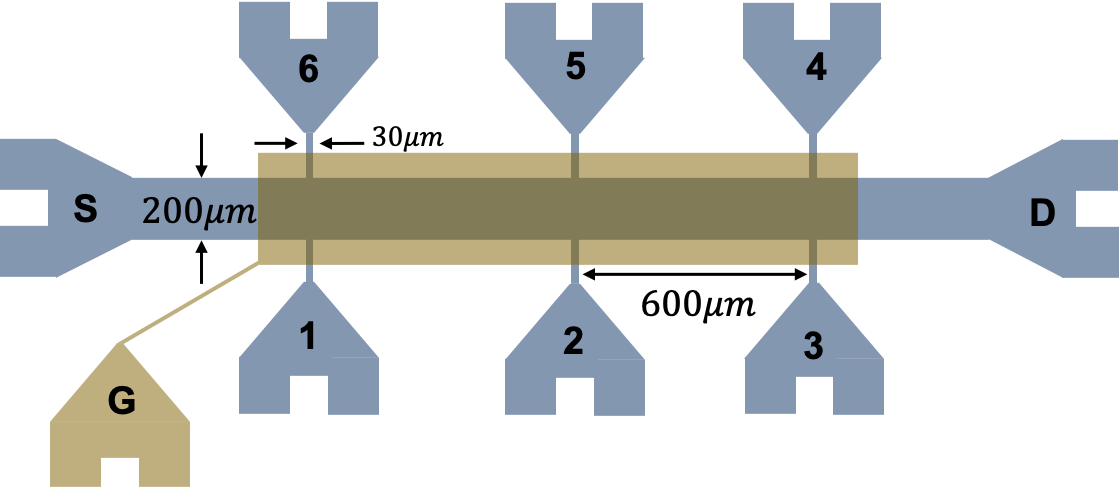
\includegraphics[width=0.45\textwidth]{../Images/HallBar.png}
    \caption{Schematic of the Hall bar geometry. The contacts are labeled with "S" for source, "D" for drain,
    "G" for gate. Contacts $4$ and $6$ are used for the measurement of the longitudinal resistance 
    and contacts $3$ and $4$ are used for the measurement of the transversal resistance.}
    \label{fig:HallBar}
\end{figure}
An AC voltage is applied between source and drain to control the longitudinal current $I$
flowing through the sample. $I$ can be measured via the voltage drop $U_\text{I}$ over a known resistor $(R_\text{S}=4.982\pm0.0005)\,\text{k}\Omega$, 
which is connected in series to the source contact. $U_\text{I}$ is measured with a Lock In amplifier 
\emph{Stanford Research Systems SR510}. Contacts $3$ and $4$ are used to measure the hall voltage $U_\text{Hall}$, which
is measured with a second Lock In amplifier of the same type. Contacts $4$ and $6$ are used to measure
the longitudinal Voltage $U_\text{xx}$, which is measured with a third Lock In amplifier \emph{Stanford Research Systems SR530}.
All Lock In amplifiers use a phase sensitive amplification approach by filtering the the noise through multiplying the signal
with a $13\,\text{Hz}$ reference signal. Moreover, the data is integrated over a period of $3\,\text{s}$ and measured with a sensitivity of $1\,\text{mV}$.
The gain accuracy is $1\%$.
The hall bar sample has a width of $200\,\mu\text{m}$ and a length of $1.2\,\text{mm}$, which can be seen in fig.\,\ref{fig:HallBar}.
For observation of the hall effect, a magnetic field $B$ is applied perpendicular to the plane of the sample.
The magnetic field is generated by a superconducting NbTi solenoid, which is cooled with liquid helium and can
be precisely controlled by the current flowing through the magnet. The flux density $B$ is read out as a voltage
$U_\text{B}$ with $U_\text{B}=10\,\text{V}$ corresponding to $9\,\text{T}$. 
The Hall bar is placed inside a variable temperature insert (VTI), 
which allows to cool down the sample by evaporating liquid He at different pressures. 
The measurements are taken at the temperatures $\csname tempFor4.2K\endcsname$, 
$\csname tempFor3K\endcsname$, $\csname tempFor2.1K\endcsname$, $\csname tempFor1.4K\endcsname$, which will be referred as the goal temperatures
$4.2K$, $3K$, $2.1K$ and $1.4K$ respectively.
The temperature of the sample is measured via the voltage drop over a $Alan Bradley$ resistor 
$R_\text{AB}=100\,\Omega$ using a \emph{Keithley 160B} digital multimeter and a constant current of $10\mu\text{m}$.
Acting as a resistive thermometer the carbon resistor is located with the sample inside the VTI and is calibrated for the used temperature range.
The conversion of Voltage to Temperature is done with the calibration table \cite{ExperimentDescription}.
The temperatures could not be stabilized perfectly, so the mean temperature between the beginning and the end of the measurement is taken.
While the magnetic field is turned on, the temperature could not be measured, since the resistor is dependent on the magnetic field.
Since the resistor is not exactly positioned at the Hall bar and its error is not known, the error in temperature is estimated to be $1\%$.
If half of the drift in temperature is larger, half of the drift is used as error. 



\section{Von Klitzing Constant}

The Hall resistivity $\rho_{\text{xy}}$ forms plateaus at
\begin{align}
    \rho_{xy} = \frac{h}{\nu e^2} =: \frac{R_\text K}{\nu}
\end{align}
with the elementary charge $e$ and the planc constant $h$. 
The filling factor $\nu \in \mathbb N$ describes the number of occupied Landau levels.
The goal of this section is to determine the von Klitzing constant $R_K$.
Before reading off the plateaus, two errors have to be taken into account:
the time delay and the different scales of the lock in amplifiers.
To account for the time delay, 
caused by the integration and perhhaps some additional internal delay of the lock in amplifiers,
the three voltages given by the lock in amplifiers are shifted backwards in time.
Since the magnetic field B is ramped up and down between $0T$ and $9T$, 
the constant shift in time can be chosen, s.t. both graphs match.
To compensate for different scales $\alpha_i$, 
the lock in amplifiers $1$ and $2$ measuring $U_\text{xy}$ and $U_\text I$ are exchanged and the measurement at $1.4\,K$ is repeated.
If $U$ and $I$ are the real values,
\begin{align}
    R_{\text K,1} = \frac{U_{\text{xy}, 1}}{I_2} = \frac{\alpha_1 U}{\alpha_2 I}\\
    R_{\text K,2} = \frac{U_{\text{xy}, 2}}{I_1} = \frac{\alpha_2 U}{\alpha_1 I}
\end{align}
one finds the correction factor
\begin{align}
    \alpha = \frac{\alpha_1}{\alpha_2} = \sqrt{\frac{U_{\text{xy},1}I_2}{U_{\text{xy}, 2}I_1}}. 
\end{align}
All further calculations are corrected for the time delay and the different scales.
Only $\rho_{\text{xy}}$ is corrected with the factor $\alpha$, 
since no additional measurement with exchanged lock in amplifiers was performed.
In principle, $\rho_{\text{xx}}$ could be corrected in the same manner.
\\
To obtain $R_\text K$, the average values of the resistivities of the plateaus is taken.
The transversal resistivity $\rho_{\text{xy}}$ of the plateaus and the resulting $R_\text K$ are presented in 
tab. \ref{tab:plateau_values} and tab. \ref{tab:Klitzing} respectively.
The error is obtained by propagating the accuracy of the lock in amplifiers.
\begin{table}[h!]
    \centering
    \begin{tabular}{c|c c c c}
        $\nu$  & $4.2\,\text{K}$        & $3.0\,\text{K}$        & $2.1\,\text{K}$        & $1.4\,\text{K}$        \\ \hline
        1      & $\csname PlateauNr14.2K\endcsname$  & $\csname PlateauNr13K\endcsname$  & $\csname PlateauNr12.1K\endcsname$  & $\csname PlateauNr11.4K\endcsname$  \\ 
        2      & $\csname PlateauNr24.2K\endcsname$  & $\csname PlateauNr23K\endcsname$  & $\csname PlateauNr22.1K\endcsname$  & $\csname PlateauNr21.4K\endcsname$  \\ 
        3      & $\csname PlateauNr34.2K\endcsname$  & $\csname PlateauNr33K\endcsname$  & $\csname PlateauNr32.1K\endcsname$  & $\csname PlateauNr31.4K\endcsname$  \\ 
        4      & $\csname PlateauNr44.2K\endcsname$  & $\csname PlateauNr43K\endcsname$  & $\csname PlateauNr42.1K\endcsname$  & $\csname PlateauNr41.4K\endcsname$  \\ 
        5      & $\csname PlateauNr54.2K\endcsname$  & $\csname PlateauNr53K\endcsname$  & $\csname PlateauNr52.1K\endcsname$  & $\csname PlateauNr51.4K\endcsname$  \\ 
    \end{tabular}
    \caption{Plateaus in Hall resistivity for different temperatures and filling factors in $k\Omega$.
    The error is $1.4\%$.
    }
    \label{tab:plateau_values}
\end{table}
\begin{table}[h!]
    \centering
    \begin{tabular}{c|c c c c}
        $\nu$  & $4.2\,\text{K}$        & $3.0\,\text{K}$        & $2.1\,\text{K}$        & $1.4\,\text{K}$        \\ \hline
        1      & $\csname PlateauMalNuNr14.2K\endcsname$  & $\csname PlateauMalNuNr13K\endcsname$  & $\csname PlateauMalNuNr12.1K\endcsname$  & $\csname PlateauMalNuNr11.4K\endcsname$  \\ 
        2      & $\csname PlateauMalNuNr24.2K\endcsname$  & $\csname PlateauMalNuNr23K\endcsname$  & $\csname PlateauMalNuNr22.1K\endcsname$  & $\csname PlateauMalNuNr21.4K\endcsname$  \\ 
        3      & $\csname PlateauMalNuNr34.2K\endcsname$  & $\csname PlateauMalNuNr33K\endcsname$  & $\csname PlateauMalNuNr32.1K\endcsname$  & $\csname PlateauMalNuNr31.4K\endcsname$  \\ 
        4      & $\csname PlateauMalNuNr44.2K\endcsname$  & $\csname PlateauMalNuNr43K\endcsname$  & $\csname PlateauMalNuNr42.1K\endcsname$  & $\csname PlateauMalNuNr41.4K\endcsname$  \\ 
        5      & $\csname PlateauMalNuNr54.2K\endcsname$  & $\csname PlateauMalNuNr53K\endcsname$  & $\csname PlateauMalNuNr52.1K\endcsname$  & $\csname PlateauMalNuNr51.4K\endcsname$  \\ 
    \end{tabular}
    \caption{$R_\text K$ for different temperatures and filling factors in $k\Omega$.
    The error is $1.4\%$.
    }
    \label{tab:Klitzing}
\end{table}
To determine the von Klizing constant, measured at different temperatures, the average value for different $\nu$ is taken.
The results are shown in tab \ref{tab:Klitzing2}.
\begin{table}[h!]
    \centering
    \begin{tabular}{c|c}
        $T\,/\,K$  & $R_\text K \, / \, k\Omega$  \\ \hline
        4.2      & $\csname Klitzing4.2K\endcsname$  \\ 
        3.0      & $\csname Klitzing3K\endcsname$   \\ 
        2.1      & $\csname Klitzing2.1K\endcsname$   \\ 
        1.4      & $\csname Klitzing1.4K\endcsname$  \\ 
    \end{tabular}
    \caption{Von Klitzing constant $R_\text K$ measured at different temperatures.
    }
    \label{tab:Klitzing2}
\end{table}
The results match the exact defined value of $R_\text{K, exact} = 2.581280...$. 





\section{Charge carrier density}
In the following section the determination of the carrier density $n$ is described using three different methods.
All determined carrier densities are listed in tab.\,\ref{tab:ns}.
\subsection{Charge carrier density extrapolation via classical Hall effect}
In the classical Hall effect, the charge carrier density $n_\text{slope}$ is given by 
\begin{align}
    n_\text{slope} = \frac{B}{\rho_{xy}e} = \frac{1}{e \cdot m_\text{slope}}.
    \label{eq:chargeCarrierClassicalHall}
\end{align}
with the slope $m_\text{slope}$ of the Hall resistance $\rho_{xy}$ as the regression parameter.
In our experiment, one expect to see the classical Hall effect at low magnetic fields.
As seen in fig.\,\ref{fig:KlitzingBeispielBild} the slope of the Hall resistance shows a linear behavior for small magnetic fields.
The carrier density is calculated by determining the slope $m_\text{slope}$ of the linear region using a linear regression for the data points for $B<1\,\text{T}$.
The error is calculated by Gaussian error propagation of the error of $m_\text{slope}$ obtained from the linear regression.

\subsection{Charge carrier density via Hall plateaus}
In the quantum Hall regime the carrier density can be calculated from the Hall plateaus with the corresponding filling factors $\nu$:
\begin{align} 
    n_\nu = \frac{\nu B_\nu e}{h} \label{eq:nnu} 
\end{align} 
where $B_\nu$ is the mean magnetic field at the plateau for the corresponding filling factor.
$B_\nu$ is determined by manually reading the center of each plateau, with the error of $B_\nu$ being the uncertainty of the reading. 
For higher filling factors, the plateaus become narrower and the error of the reading becomes slightly smaller, as the midpoint of the plateaus is easier to determine.
The error of $n_\nu$ is then calculated by Gaussian error propagation.

\subsection{Charge carrier density via Shoubnikow-de Haas effect}
\begin{figure}[h]
    \centering
    \includegraphics[width=0.45\textwidth]{../Images/FourierMitGausFür14K.png}
    \caption{Fourier transform of the longitudinal resistivity 
    $\mathcal{F}\left[ \rho^\prime_\text{xx}\right]\left(f_\text B\right)$ 
    for $1.4\,\text{K}$ to determine the frequency of Shoubnikow-de Haas oscillations.\\
    The peak is determined with a fit of a gaussian curve.
    }
    \label{fig:Fourier}
\end{figure}
The Shoubnikow-de Haas effect describes the oscillations of the longitudinal resistivity $\rho_{xx}$ with increasing magnetic field $B$.
It can be explained with the equally spaced Landau levels moving up in energy, when $B$ increases.
The charge carrier density $n_\text{SdH}$ is calculated via
\begin{align}
    n_\text{SdH} = \frac{e}{h\Delta}
    \label{eq:chargeCarrierFourier}
\end{align} 
with the periodicity of oscillations $\Delta\left(\frac{1}{B}\right)$.
To obtain the periodicity $\Delta$, the longitudinal resistivity $\rho^\prime_\text{xx}\left(B\right)=\rho_\text{xx}\left(\frac{1}{B}\right)$ is considered.
Since the measured data points are equally spaced in $B$ instead of $\frac{1}{B}$, an interpolation is performed.
A discrete Fast Fourier Transform is applied to accurately determine the period of the oscillations.
A clear peak is visible.
To accurately locate the peak, a Gaussian is fit to the region and the peak value of the fit is used as $\Delta$.
The error of the peak is estimated to be half the width of the Gaussian $\sigma / 2$.
The Fourier transformed resistivity $\mathcal{F}\left[ \rho^\prime_\text{xx}\right]\left(f_\text B\right)$ for $1.4\,\text{K}K$ is shown in fig. \ref{fig:Fourier}.
The charge carrier densities calculated with eq. \ref{eq:chargeCarrierFourier} are shown in tab. \ref{tab:ns}.
\begin{table}[h]
    \centering
    \begin{tabular}{c|c|c}
        \hline\hline
        Method & $T / \text{K}$ & $n\,/\,10^{15}\text{m}^{-2}$ \\\hline\hline
        slope & 4.2 & $\csname nEins4.2K\endcsname$ \\
        & 3 & $\csname nEins3K\endcsname$ \\
        & 2.1 & $\csname nEins2.1K\endcsname$ \\
        & 1.4 & $\csname nEins1.4K\endcsname $\\\hline
        $\nu$ & 4.2 & $\csname nZwei4.2K\endcsname$ \\
        & 3 & $\csname nZwei3K\endcsname$ \\
        & 2.1 & $\csname nZwei2.1K\endcsname$ \\
        & 1.4 & $\csname nZwei1.4K\endcsname$ \\\hline
        SdH & 4.2 & $\csname FourierN4.2K\endcsname$ \\
        & 3 & $\csname FourierN3K\endcsname$ \\
        & 2.1 & $\csname FourierN2.1K\endcsname$ \\
        & 1.4 & $\csname FourierN1.4K\endcsname$ \\\hline\hline
    \end{tabular}
    \caption{Data of the charge carrier density $n$ calculated with different methods.
    The values are given in units of $10^{15}\,\text{m}^{-2}$. For all following sections
    the method $n_\text{slope}$ is chosen for the determination of $n$. \label{tab:ns}}
\end{table}




\section{Fractional QHE}

Experiments show, that the filling factor $\nu$ not only takes integer values, but also fractions $\nu=\frac{1}{2}, \frac{2}{5}, ...$.
This can partially be explained with the creation of fractionally charged quasiparticles.
This effect is typically observed for very high magnetic fields.
Since none of the curves goes beyond $\nu = 1$, 
a larger magnetic field would be required to observe fractional filling factors smaller than 1.
In principle, also fractional filling factors larger that one can occur.








\section{Gate Voltage and Charge Carrier Density}
To understand the influence of different carrier densities $n$, the gate voltage $U_\text{gate}$ is varied.
A higher $U_\text{gate}$ increases the Fermi level and thus the carrier density.
Gate voltages of $1.5 \,\text V, 1 \,\text V, -0.25 \,\text V, -1 \,\text V, -1.5 \,\text V$ have been applied.
The resistivities with first three gate voltages are shown in fig. \ref{fig:differentGateVoltagesQHE}.
They show Hall plateaus and Shoubnikow-de Haas oscillations.
The Hall resistance $\rho_\text{xy}$ grows more slowly with $B$ for larger carrier densities.
Note that the plateaus in $\rho_\text{xy}$ remain at the same discrete values, but require higher $B$.
This can be explained by the higher Fermi level, which has more Landau levels below it.
A higher $B$ is required to move the Landau levels above the Fermi level.
\begin{figure}[h]
    \centering
    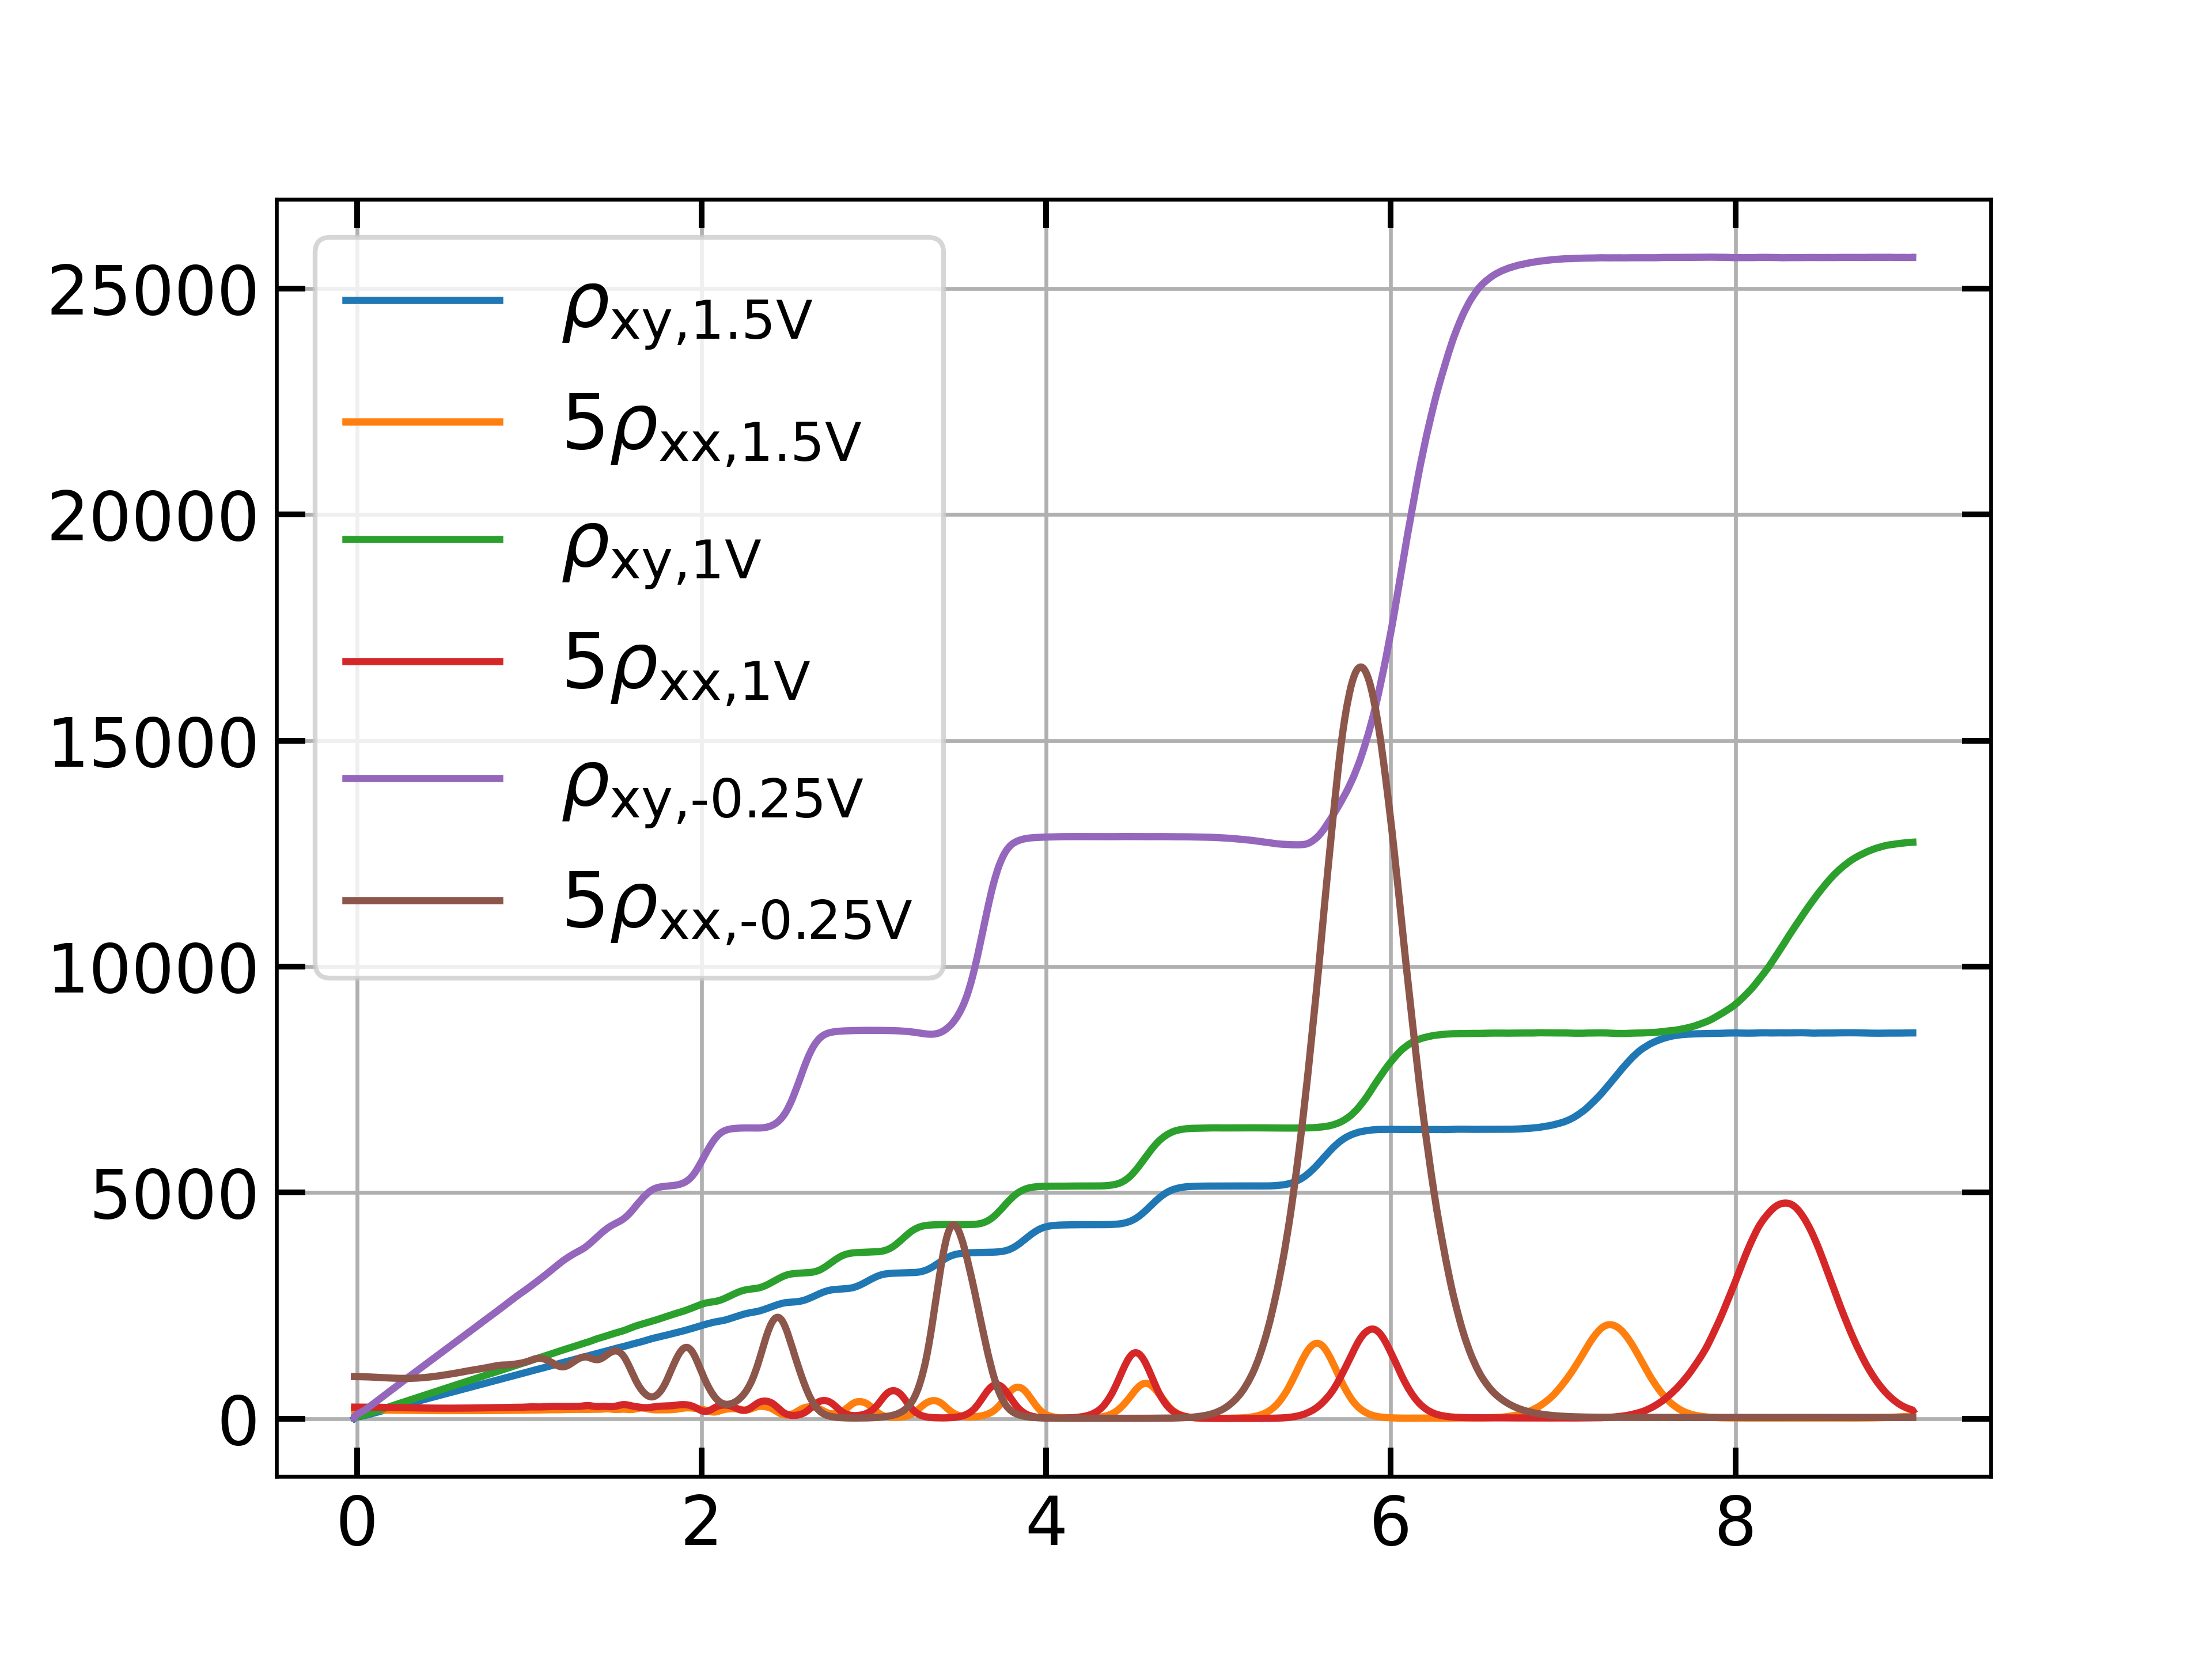
\includegraphics[width=0.45\textwidth]{../Images/differentGateVoltagesQHE.png}
    \caption{Resistivities $\rho_\text{xy}$ and $\rho_\text{xx}$ for different gate voltages at $1.4\,\text{K}$. 
    All 6 curves are in the regime of electron conduction.
    Lower $U_\text{gate}$
     leads to a steeper incline of $\rho_\text{xy}$ and higher peaks in $\rho_\text{xx}$ with larger gaps in between.
    The plateaus keep their discrete values.
}
    \label{fig:differentGateVoltagesQHE}
\end{figure}
In these three cases, the Fermi level remains above (or at, for $\nu=1$) the lowest Landau level.
Note that for fixed $n$ the lowest Landau level will not cross the Fermi level by increasing $B$.
However, the Fermi level can be shifted below the lowest Landau level if $U_\text{gate}$ and the corresponding $n$ are low enough.
Then only levels corresponding to defects will be around the Fermi level.
If $U_\text{gate}$ is lowered further, the Fermi level will cross the band gap from the conduction band to the valence band.
More Landau levels should appear, but the corresponding charge carriers are no longer electrons, but holes.
This transition is investigated with $U_\text{gate}=-1 \,\text V,\,-1.5 \,\text V$.
The resistivities for these gate voltages are plotted in fig. \ref{fig:kaputteKurvenGateV}.
\begin{figure}[h]
    \centering
    
\includegraphics[width=0.45\textwidth]{../Images/kaputteKurvenGateV.png}
    \caption{
        Resistances $\rho_\text{xy}$ and $\rho_\text{xx}$ at $1.4\text{K}$ for different gate voltages, corresponding to low carrier densities $n$.  
        The slope for small $B$ indicates the small value of $n$.
        Defects may play an important role for small $n$.
        Negative $\rho_\text{xy}$ correspond to p-type conduction, positive $\rho_\text{xy}$ to n-type conduction.}
    \label{fig:kaputteKurvenGateV}
\end{figure}
For the gate voltage of $1\,\text V$ the carrier density is very low, resulting in the steep slope of $\rho_\text{xy}$.
This explains why the plateau corresponding to $\nu = 1$ is already reached at $B\approx1.6 \,\text T$ and the plateaus corresponding to $\nu > 1$ are not visible.
The longitudinal component has vanishing resistivity for values of $B$ where $\rho_\text{xy}$ is constant.
For these small carrier densities, defects with localized states could play an increasingly important role.
After further increasing $B$, $\rho_\text{xy}$ temporarily shows negative values.
This could be explained by p-type conduction, 
since the holes with positive charges moving in the opposite direction are deflected in the same direction by Lorentz force as the electrons, resulting in a sign change of $\rho_\text{xy}$.
Since the valence band typically has a smaller curvature near the band gap, the holes typically have a larger effective mass $m^\ast$.
The cyclotron frequency
\begin{align}
    \omega_c = \frac{eB}{m^\ast}    
\end{align}
an therefore the energy (difference) of the Laudau levels
\begin{align}
    \epsilon = \hbar \omega_c \left(\frac{1}{2} + n_\text L \right)
\end{align}
is smaller for the holes.
This makes the Landau levels more difficult to separate. 
Larger $B$ would be needed to get the same results as with electrons.
The $\rho_\text{xy}$ of $U_\text{gate} = -1.5\,\text V$ has a negative slope for small $B$.
This is interpreted as p-type conduction, resulting in a negative carrier density.
Note that the transverse conductivity does not vanish for $B=0$.
This could be a sign of anisotropy in the material.
It is unclear why this shift only applies to holes.
$\rho_\text{xy}$ for $U_\text{gate} = -1.5 \,\text V$ does not reach the von Klitzing constant.
It is assumed that even lower $U_\text{gate}$ will show plateaus.

Extrapolating $n$ for lower $U_\text{gate}$ gives an estimate for the charge carrier density (see fig. \ref{fig:extrapolating}).
\begin{figure}[h]
    \centering
    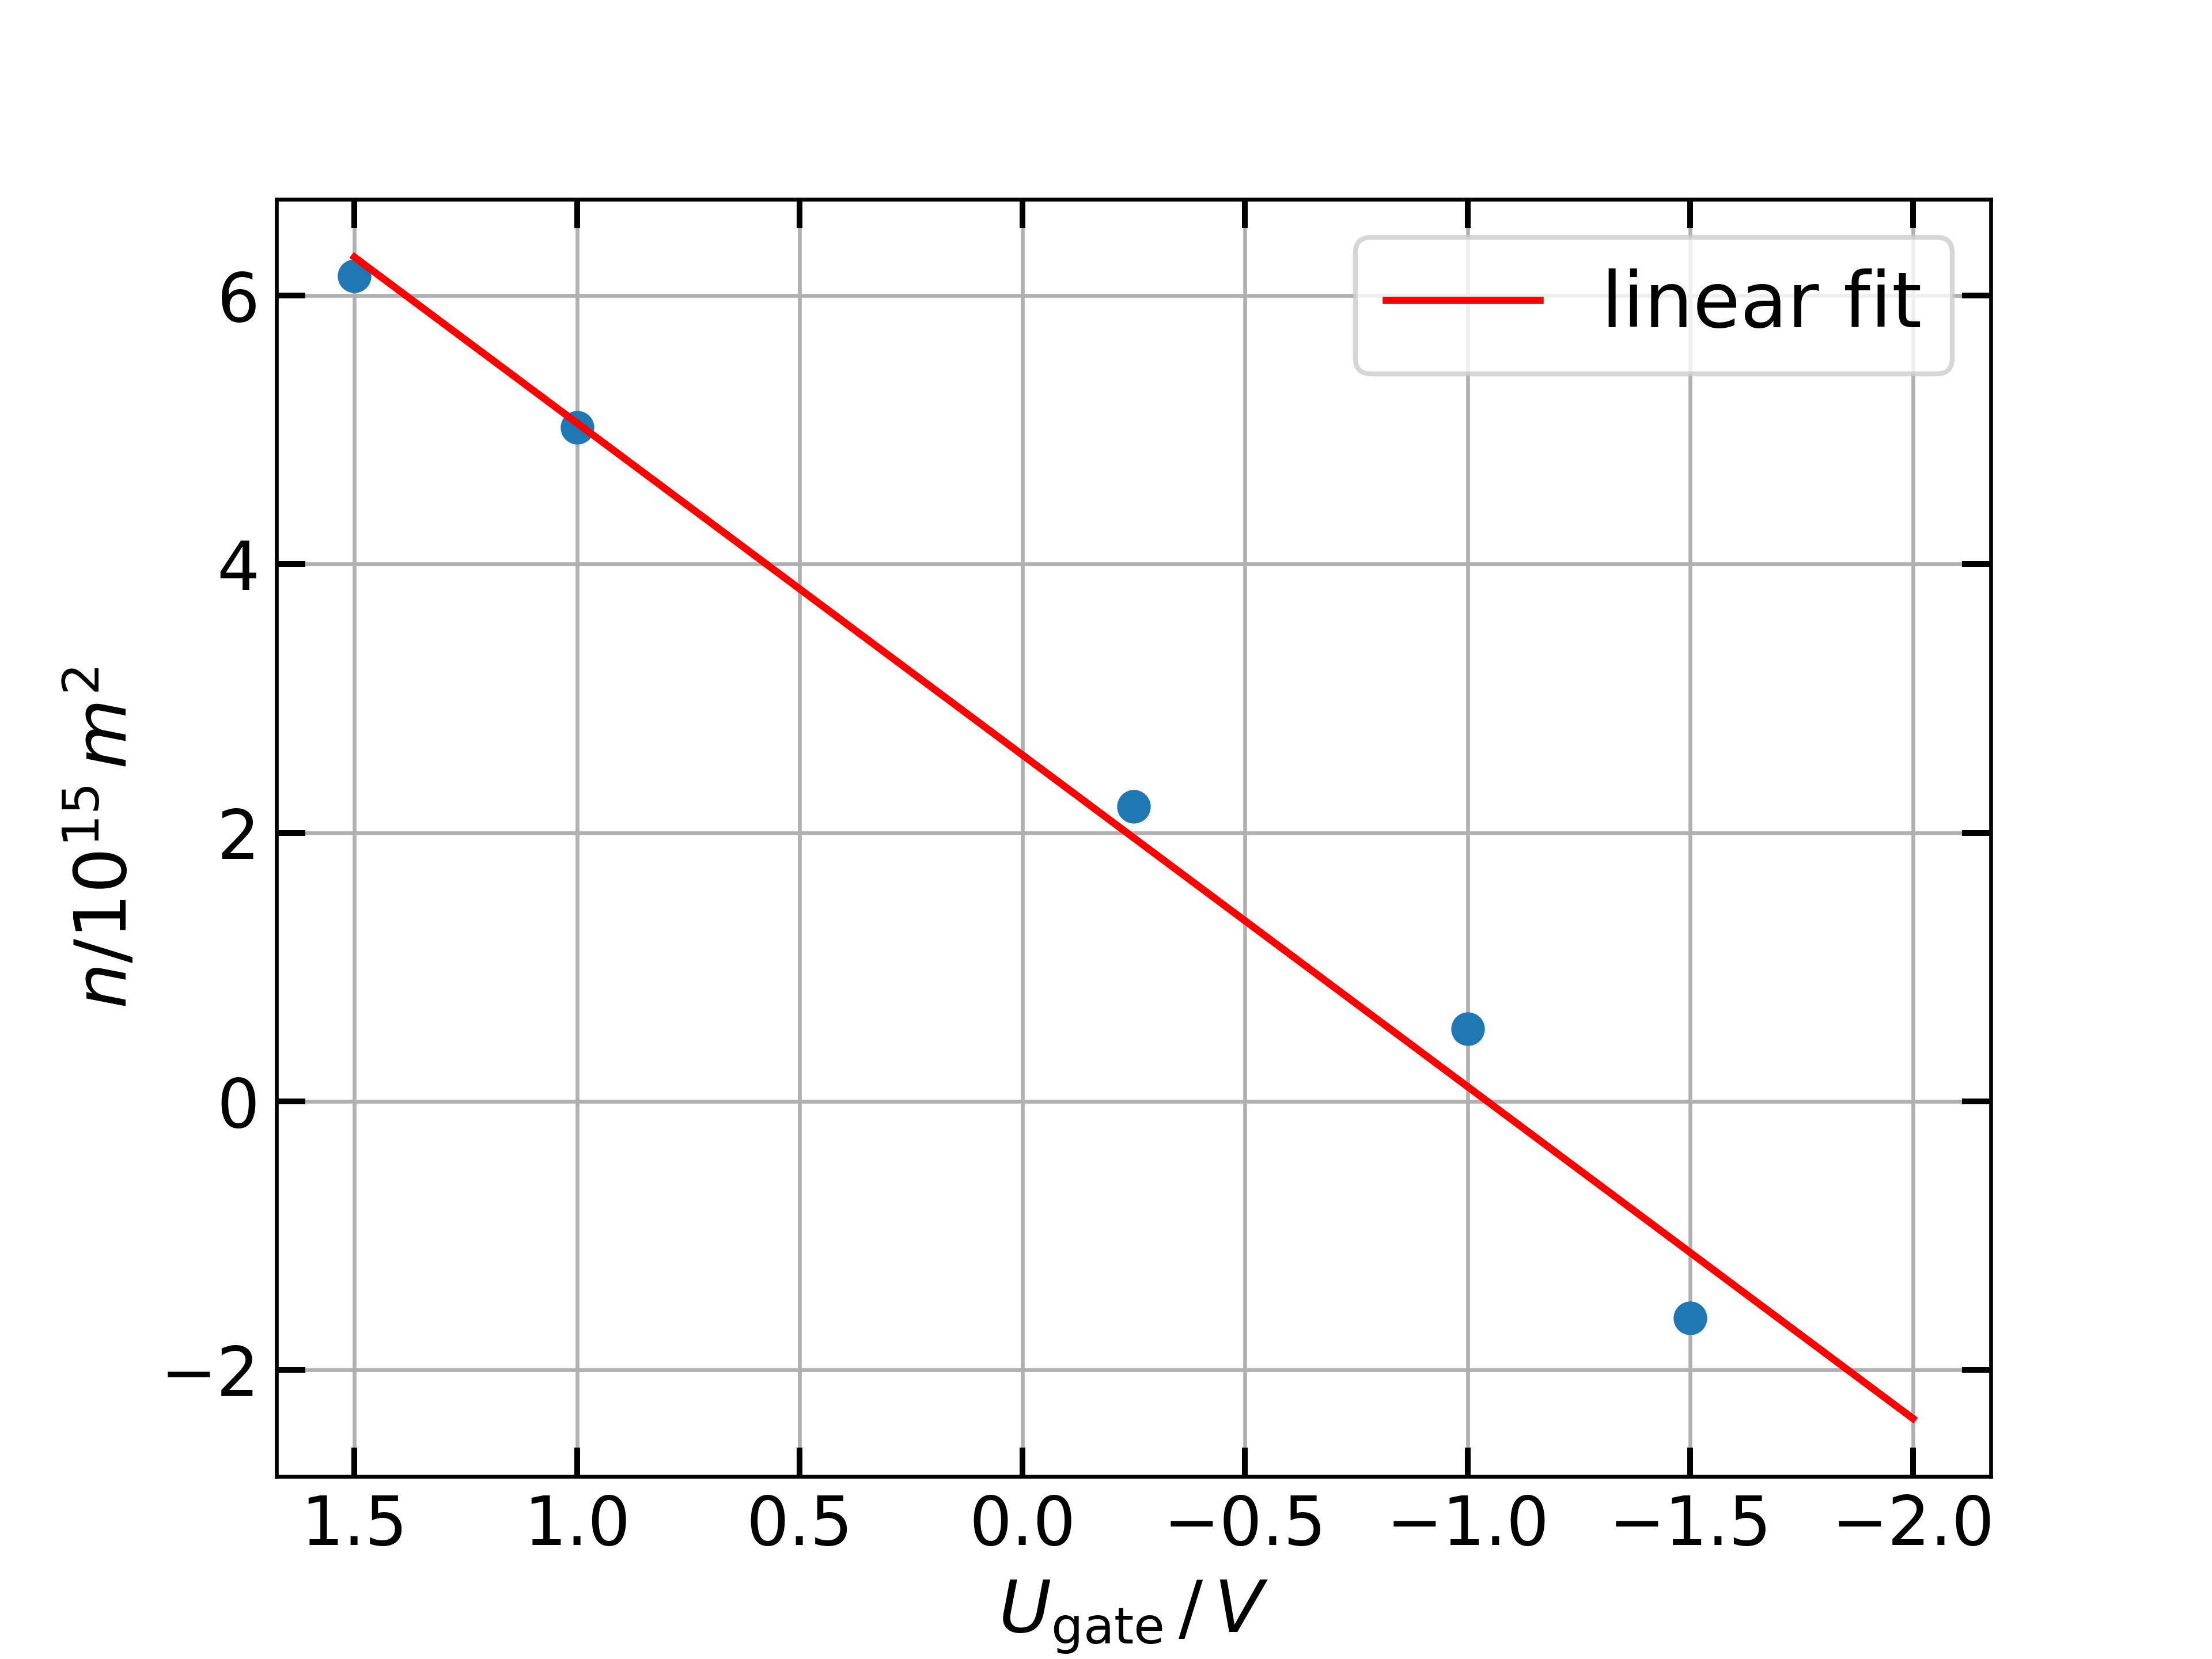
\includegraphics[width=0.45\textwidth]{../Images/extrapolatingN.png}
    \caption{
        Dependence of charge carrier density $n$ on gate voltage.
        The linear fit is extrapolated to estimate the gate voltage required to have a hole carrier density comparable to the electron carrier density with $U_\text{gate} = -0.25\,\text{V}$.}
    \label{fig:extrapolating}
\end{figure}
To obtain a hole carrier density comparable to the electron carrier density for $U_\text{gate} = -0.25\,\text{V}$,
a gate voltage of $U_\text{gate} \approx -2\,\text V$ is required.


\newpage
\begin{thebibliography}{99}
    \bibitem{Nobelpreis} K. von Klitzing, G. Dorda, and M. Pepper, \emph{New Method for High-Accuracy
    Resistance Standard Based on Quantized Hall Resistance}, Phys. Rev. Lett. \textbf{45}, 494 (1980).
    \bibitem{ExperimentDescription} ja kommt noch

    \bibitem{klitzing}CODATA. (2018). CODATA recommended values of the fundamental physical constants: 
    2018. NIST Physical Measurement Laboratory.
    https://physics.nist.gov/cgi-bin/cuu/Value?rk



\end{thebibliography}




\end{document}
